\documentclass[11pt,twocolumn]{article}

% ---- packages ----
\usepackage[utf8]{inputenc}
\usepackage[T1]{fontenc}
\usepackage{times}
\usepackage[margin=0.85in]{geometry}
\usepackage{graphicx}
\usepackage{booktabs}
\usepackage{amsmath}
\usepackage{hyperref}
\usepackage{xcolor}
\usepackage{caption}
\usepackage{natbib}
\usepackage{enumitem}
\usepackage{microtype}
\usepackage{titlesec}

% ---- style ----
\hypersetup{colorlinks=true, linkcolor=blue!60!black, citecolor=blue!60!black, urlcolor=blue!60!black}
\captionsetup{font=small, labelfont=bf, skip=6pt}
\setlength{\columnsep}{0.3in}
\titlespacing*{\section}{0pt}{10pt}{5pt}
\titlespacing*{\subsection}{0pt}{8pt}{4pt}
\setlist{nosep, leftmargin=1.2em}

% ---- title ----
\title{\textbf{FACET: Measuring Attribution Faithfulness\\in Multi-Factor LLM Reasoning}}

\author{
  \textbf{Venkateshwar Reddy Jambula} \\
  Pranaalpha Labs \\
  \texttt{venkateshwar.jambula@pranaalpha.com}
}

\date{April 2026}

\begin{document}
\twocolumn[
  \maketitle
  \begin{@twocolumnfalse}
  \begin{abstract}
  \noindent
  Many decisions require weighing $N \geq 5$ different factors simultaneously. When LLMs are deployed in these settings, do they integrate all factors or collapse onto whichever one is most canonical in their training data? We present \textbf{FACET} (Factor Accessibility, Coverage, and Evidence Test), a pilot study using a \emph{counterfactual-outcome protocol}: neutralize the canonical factor and flip the remaining factors, creating cases where integration and single-factor processing predict different outcomes. We test nine frontier configurations (eight in the counterfactual arm) from six labs on US tort law (chosen for explicit factor lists and verifiable ground truth). All models answer correctly on counterfactuals, but \textbf{probe faithfulness varies by canonicity}: 7/8 models update their attribution when a moderately canonical factor is neutralized, \textbf{0/8 update for a highly canonical factor}, and 4/8 for an intermediate case. We interpret this as \emph{canonicity-dependent embedding strength} and connect it to \citet{turpin2023} on chain-of-thought unfaithfulness. The protocol is not specific to law; legal balancing tests are the first instantiation.
  \end{abstract}
  \vspace{12pt}
  \end{@twocolumnfalse}
]

%==============================================================
\section{Introduction}
%==============================================================

\subsection{The Problem}

Many decisions require weighing $N \geq 5$ qualitatively different factors against one another: a physician balancing symptoms, lab results, and patient history; a compliance officer weighing risk indicators across regulatory dimensions; a judge integrating doctrinal factors in a balancing test. When LLMs are deployed in these settings, a core question arises: \emph{does the model actually integrate all $N$ factors, or does it collapse onto whichever single factor is most canonical in its training data?}

Both strategies can produce the same correct answer on typical cases, so outcome accuracy alone cannot distinguish them. The key methodological challenge is constructing cases where the two strategies predict different outcomes.

\subsection{Why Legal Balancing Tests}

We instantiate FACET in the domain of US tort law because legal balancing tests offer three properties that make them an ideal testbed for multi-factor reasoning:

\begin{enumerate}
\item \textbf{Explicit factor lists.} Doctrines like \emph{Rowland v.\ Christian} (1968, seven factors for duty of care), \emph{Barker v.\ Lull Engineering} (1978, five factors for design defect), and \emph{Biakanja v.\ Irving} (1958, six factors for third-party duty) enumerate their factors by name. This eliminates ambiguity about what the model should be weighing.
\item \textbf{Verifiable ground truth.} Appellate court holdings provide an externally adjudicated correct answer, unlike most multi-factor domains where ground truth is debatable.
\item \textbf{Varying canonicity.} Some factor-doctrine associations are deeply canonical in training data (every torts textbook frames Barker as ``the feasible-alternative-design case''), while others are more diffuse. This variation lets us test whether training-data canonicity predicts attribution faithfulness.
\end{enumerate}

The methodology---neutralize the canonical factor, flip the remaining factors, measure whether the model's attribution updates---applies to any domain with explicit multi-factor structure. Legal balancing tests are the first instantiation; medical differential diagnosis and multi-criteria compliance review are planned extensions (Section~7).

\subsection{Prior Art}

The cognitive-science literature on multi-attribute decision making distinguishes two strategies \citep{payne1993}: \textbf{WADD} (weighted additive---integrate all attributes weighted by their importance) and \textbf{LEX} (lexicographic---pick the single most important attribute and decide based on that alone). \citet{lieder2020} reframed LEX as rational under limited cognitive resources.

Existing LLM benchmarks on legal reasoning---LegalBench \citep{guha2023}, LEXam \citep{katz2025}, MSLR \citep{yu2025}---evaluate outcome correctness but none directly probe whether the model is integrating factors or collapsing. The closest neighbor is \citet{zhang2025} on hierarchical CATO factor reasoning in trade-secret law, which tests \emph{sequential} factor roll-up; FACET tests \emph{parallel} integration at the final balancing step.

The chain-of-thought unfaithfulness literature \citep{turpin2023,lanham2023} established that LLM reasoning traces do not always reflect the causal process that produced the answer. FACET connects to this line of work but measures a different signal: direct-probe factor attribution rather than reasoning-trace faithfulness.

\subsection{Contributions}

\begin{enumerate}
\item \textbf{A counterfactual protocol} for measuring attribution faithfulness in multi-factor reasoning. Neutralize the canonical factor, reverse the remaining factors, and measure whether the model's self-reported attribution updates.
\item \textbf{A pilot dataset} of ten real legal balancing cases across three doctrinal frameworks, plus three counterfactual variants.
\item \textbf{Canonicity-dependent probe dissociation.} Probe faithfulness varies by how deeply a factor-domain association is embedded in training data (7/8, 0/8, 4/8 across three canonicity levels) rather than by model family.
\item \textbf{A negative result on inference-time compute.} Extended thinking on Claude Opus 4.6 does not reduce probe dissociation.
\item \textbf{An open harness and dataset} for replication.
\end{enumerate}

%==============================================================
\section{Multi-Factor Collapse and Probe Dissociation}
%==============================================================

We operationalize multi-factor collapse via five necessary conditions:
\begin{enumerate}
\item \textbf{Co-present, not sequentially introduced.} All $N$ factors are present in the model's input at the start.
\item \textbf{Different in kind.} Factors span qualitatively different categories.
\item \textbf{Integrative, not dominated.} No single factor carries more than 0.5 of the decision weight.
\item \textbf{Semantically retrievable.} The model can reproduce each factor when probed.
\item \textbf{Behaviorally indistinguishable from LEX under perturbation.}
\end{enumerate}

We define \textbf{probe dissociation} as a condition where the model reaches the correct outcome but reports a factor attribution inconsistent with the case facts---specifically, identifying a neutralized factor as ``most important.''

%==============================================================
\section{Method}
%==============================================================

\subsection{In-Distribution Instances}

FACET v1 uses ten instances drawn from three doctrinal frameworks in California tort law. The three anchor instances are:

\begin{itemize}
\item \textbf{Cabral v.\ Ralphs Grocery Co.}, 51 Cal.\ 4th 764 (2011). Rowland seven-factor duty analysis. Unanimous: duty exists.
\item \textbf{Barker v.\ Lull Engineering}, 20 Cal.\ 3d 413 (1978). Five-factor risk-benefit prong of design defect. Unanimous: design-defect theory viable.
\item \textbf{Biakanja v.\ Irving}, 49 Cal.\ 2d 647 (1958). Six-factor duty-to-third-party. Unanimous: duty exists.
\end{itemize}

Seven additional instances bring the total to ten. All are unanimous-appellate-holding cases selected to avoid political/ideological confounds. Factor definitions and ground-truth holdings are sourced from secondary legal digests; verification against primary opinion texts is ongoing and will be completed before any conference submission. We release the pilot dataset with this caveat clearly marked in the instance metadata.

\subsection{Counterfactual-Outcome Instances}

For each anchor doctrine, we construct a synthetic counterfactual variant designed to produce different predictions under WADD and LEX:

\begin{itemize}
\item \textbf{CF-Cabral:} F1 (foreseeability) neutralized; six other factors rewritten to point against duty. Ground truth: no duty.
\item \textbf{CF-Barker:} F3 (feasibility of a safer alternative design) neutralized; four other factors rewritten against liability. Ground truth: no design defect.
\item \textbf{CF-Biakanja:} F1 (intent-to-affect) neutralized; five other factors rewritten against duty. Ground truth: no duty.
\end{itemize}

Under WADD, the aggregate of $N{-}1$ opposing factors overwhelms one neutralized factor. A LEX-locked model that depends on the canonical factor may default to the base-case training prior, producing the wrong answer. Figure~\ref{fig:protocol} illustrates the protocol.

\begin{figure*}[t]
\centering
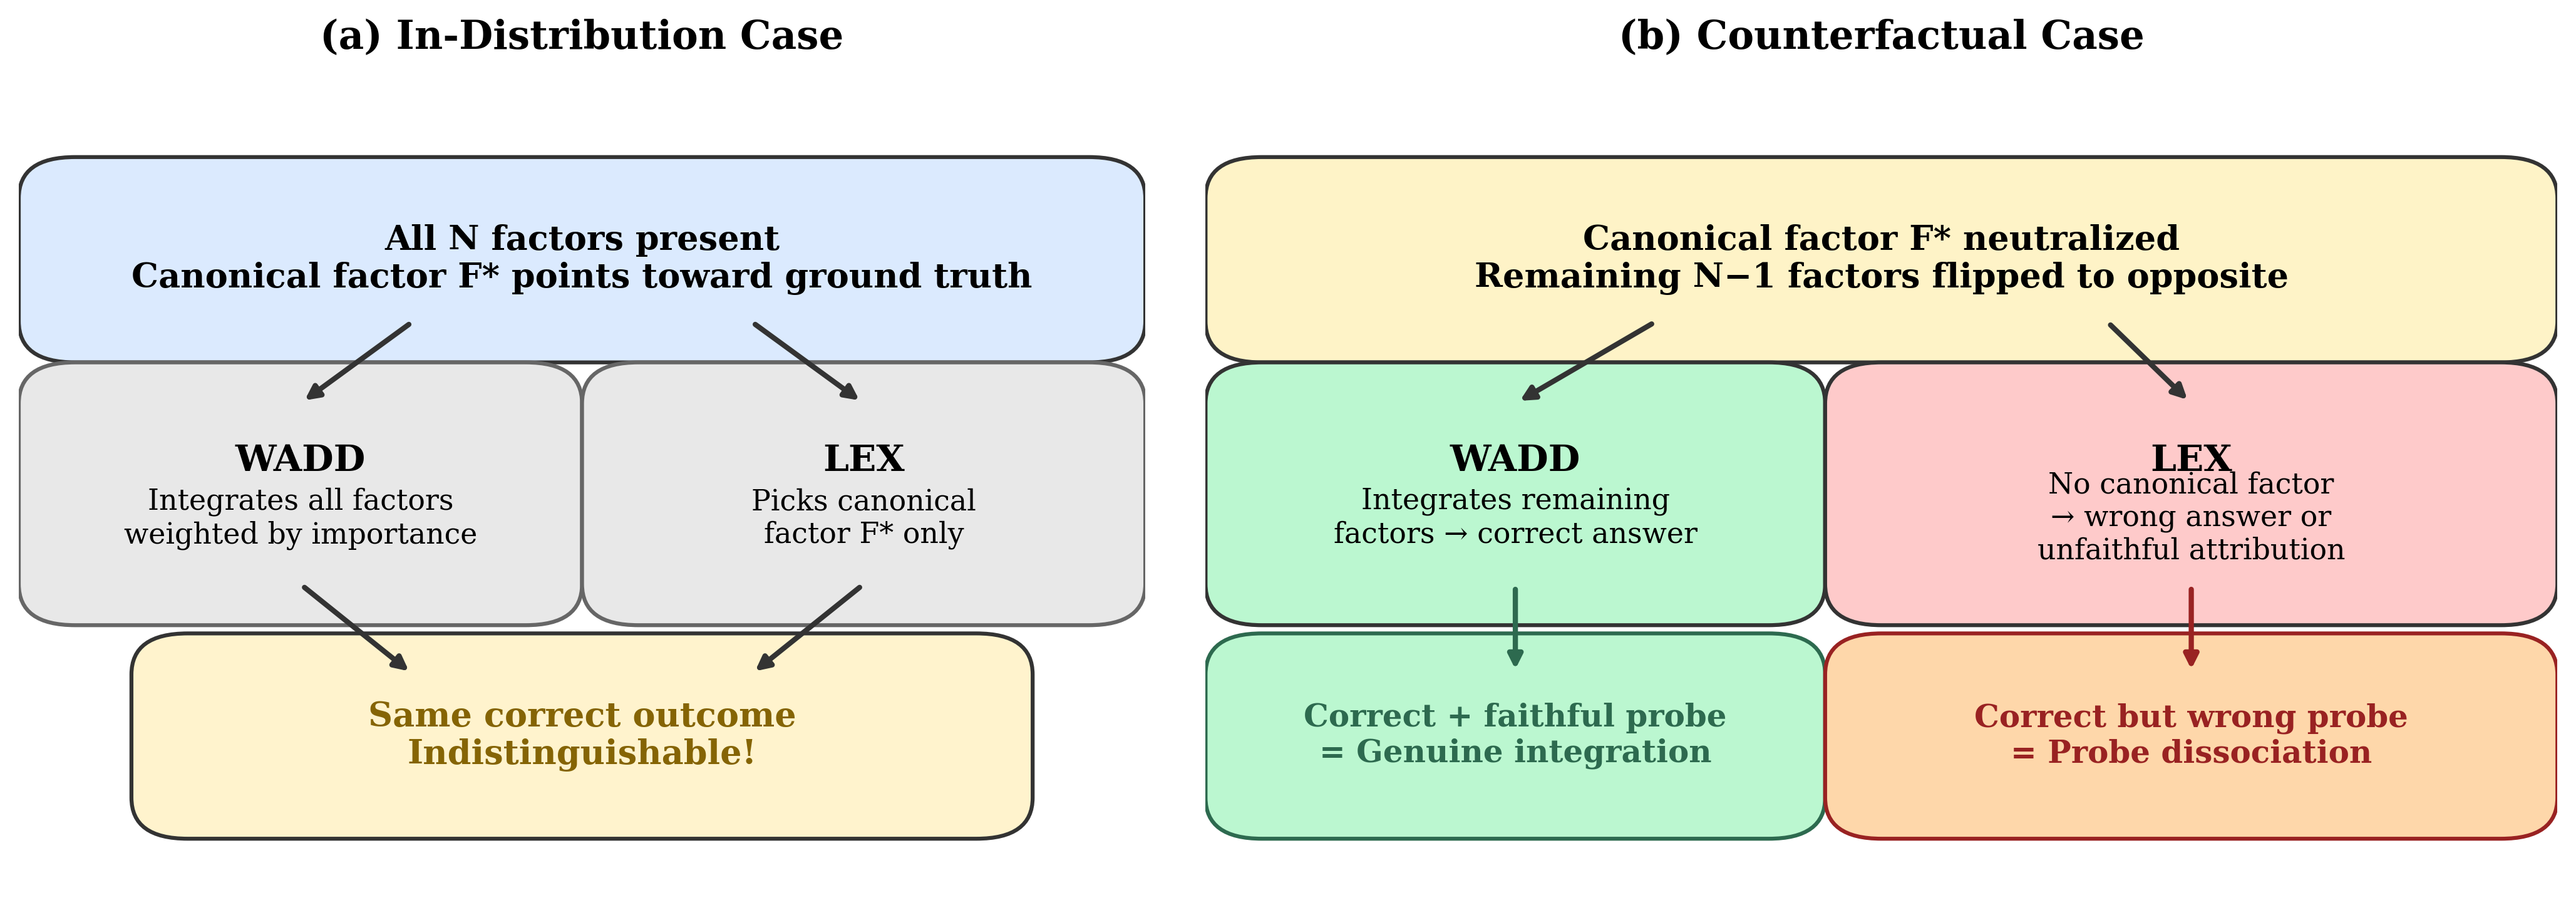
\includegraphics[width=0.85\textwidth]{fig3_protocol.png}
\caption{The counterfactual protocol distinguishes three outcomes: LEX-locked failure (wrong answer), probe dissociation (correct answer but unfaithful attribution), and genuine WADD integration (correct answer with faithful attribution).}
\label{fig:protocol}
\end{figure*}

\subsection{Conditions}

Each in-distribution instance is run under three conditions:
\begin{itemize}
\item \textbf{C0 (base integration):} All $N$ factors presented; the model produces an answer and responds to a direct probe.
\item \textbf{C2 (weight-perturbation):} For each factor $i$, rewrite factor $i$'s text to a doctrinally neutral value and re-run.
\item \textbf{C3 (compliance-matched parallel):} Factors rephrased as independent yes/no compliance requirements.
\end{itemize}

Counterfactual instances are run under C0 only. Claude Opus 4.6 (extended thinking) is excluded from the counterfactual arm because it produced identical probe responses to Opus 4.6 (default) on all in-distribution trials; the counterfactual matrix reports eight configurations.

\subsection{Models}

Nine frontier configurations across six labs (Table~\ref{tab:models}). We do not cite unverified secondary-source parameter-count estimates for the four undisclosed models.

\begin{table}[t]
\centering
\caption{Model configurations evaluated.}
\label{tab:models}
\small
\begin{tabular}{@{}llr@{}}
\toprule
\textbf{Lab} & \textbf{Model} & \textbf{Params} \\
\midrule
Anthropic & Claude Sonnet 4.6 & n/d \\
Anthropic & Claude Opus 4.6 & n/d \\
Anthropic & Opus 4.6 (ext.\ think.) & n/d \\
OpenAI & GPT-5.4 & n/d \\
Mistral & Large 3 & 675B/41B \\
DeepSeek & v3.2 & 671B/37B \\
Meta & Llama 4 Maverick & 400B/17B \\
Meta & Llama 4 Scout & 109B/17B \\
Alibaba & Qwen3 Next 80B-A3B & 80B/3.9B \\
\bottomrule
\end{tabular}
\end{table}

%==============================================================
\section{Results}
%==============================================================

\subsection{In-Distribution Results}

Table~\ref{tab:indist} reports the in-distribution results on three anchor instances. All 27 anchor-instance-model combinations reach the correct ground-truth outcome. Cross-family consensus on the canonical factor is strong but varies by doctrine: 8/9 agree on F1 (foreseeability) for Rowland, 6/9 agree on F3 (feasibility of a safer alternative design) for Barker, and 7/9 agree on F1 (intent-to-affect) for Biakanja. Probe shifts are rare: across 177 valid C2 trials, only 29 (16\%) produced a shift. Claude Opus 4.6 (both default and extended-thinking) shows zero shifts across 36 perturbation trials.

\begin{table}[t]
\centering
\caption{In-distribution results on three anchor instances. All outcomes correct. ``Shifts'' = probe changes under C2 perturbation. ``Cons.'' = consensus match.}
\label{tab:indist}
\small
\setlength{\tabcolsep}{3pt}
\begin{tabular}{@{}lccc c@{}}
\toprule
\textbf{Model} & \textbf{Cabral} & \textbf{Barker} & \textbf{Biakanja} & \textbf{Cons.} \\
\midrule
Sonnet 4.6 & F1, 1/7 & F3, 1/5 & F1, 1/6 & 3/3 \\
Opus 4.6 & F1, 0/7 & F3, 0/5 & F1, 0/6 & 3/3 \\
Opus (ext.) & F1, 0/7 & F3, 0/5 & F1, 0/6 & 3/3 \\
GPT-5.4 & F1, 0/7 & F3, 2/4 & F1, 1/6 & 3/3 \\
Mistral L3 & F1, 1/7 & F3, 1/5 & F1, 2/6 & 3/3 \\
DeepSeek v3.2 & F1, 0/7 & F3, 1/5 & F1, 1/6 & 3/3 \\
Maverick & F1, 0/7 & F1, 1/5 & F4, 3/6 & 1/3 \\
Scout & F5, 2/7 & F1, 1/5 & F6, 4/6 & 0/3 \\
Qwen3 Next & F1, 1/7 & F1, 1/4 & F1, 1/5 & 2/3 \\
\bottomrule
\end{tabular}
\end{table}

\subsection{Counterfactual Probe-Faithfulness Matrix}

Table~\ref{tab:cf} and Figure~\ref{fig:heatmap} report the counterfactual results. All 24 model-instance combinations reach the correct WADD-consistent outcome.

Probe faithfulness varies sharply by doctrine:
\begin{itemize}
\item \textbf{CF-Cabral (F1 neutralized):} 7/8 faithful. Only Maverick reports the neutralized foreseeability factor.
\item \textbf{CF-Barker (F3 neutralized):} 0/8 faithful. Every model reports the neutralized factor as most important despite explicit neutralization.
\item \textbf{CF-Biakanja (F1 neutralized):} 4/8 faithful. Claude, GPT-5.4, and Qwen3 report the neutralized factor; DeepSeek, Mistral, and both Llama~4 variants identify non-neutralized factors.
\end{itemize}

\begin{table}[t]
\centering
\caption{Counterfactual probe-faithfulness matrix. \colorbox{green!20}{Green} = faithful (non-neutralized factor identified). \colorbox{red!20}{Red} = dissociation (neutralized factor identified).}
\label{tab:cf}
\small
\setlength{\tabcolsep}{3pt}
\begin{tabular}{@{}l ccc c@{}}
\toprule
 & \textbf{CF-Cab.} & \textbf{CF-Bar.} & \textbf{CF-Bia.} & \\
\textbf{Model} & \textbf{(F1 n.)} & \textbf{(F3 n.)} & \textbf{(F1 n.)} & \textbf{Score} \\
\midrule
Sonnet 4.6 & \colorbox{green!20}{F5} & \colorbox{red!20}{F3} & \colorbox{red!20}{F1} & 1/3 \\
Opus 4.6 & \colorbox{green!20}{F6} & \colorbox{red!20}{F3} & \colorbox{red!20}{F1} & 1/3 \\
GPT-5.4 & \colorbox{green!20}{F6} & \colorbox{red!20}{F3} & \colorbox{red!20}{F1} & 1/3 \\
DeepSeek v3.2 & \colorbox{green!20}{F6} & \colorbox{red!20}{F3} & \colorbox{green!20}{F2} & 2/3 \\
Mistral L3 & \colorbox{green!20}{F5} & \colorbox{red!20}{F3} & \colorbox{green!20}{F4} & 2/3 \\
Maverick & \colorbox{red!20}{F1} & \colorbox{red!20}{F3} & \colorbox{green!20}{F3} & 1/3 \\
Scout & \colorbox{green!20}{F5} & \colorbox{red!20}{F3} & \colorbox{green!20}{F6} & 2/3 \\
Qwen3 Next & \colorbox{green!20}{F3} & \colorbox{red!20}{F3} & \colorbox{red!20}{F1} & 1/3 \\
\midrule
\textbf{Faithful} & \textbf{7/8} & \textbf{0/8} & \textbf{4/8} & \\
\bottomrule
\end{tabular}
\end{table}

\begin{figure*}[t]
\centering
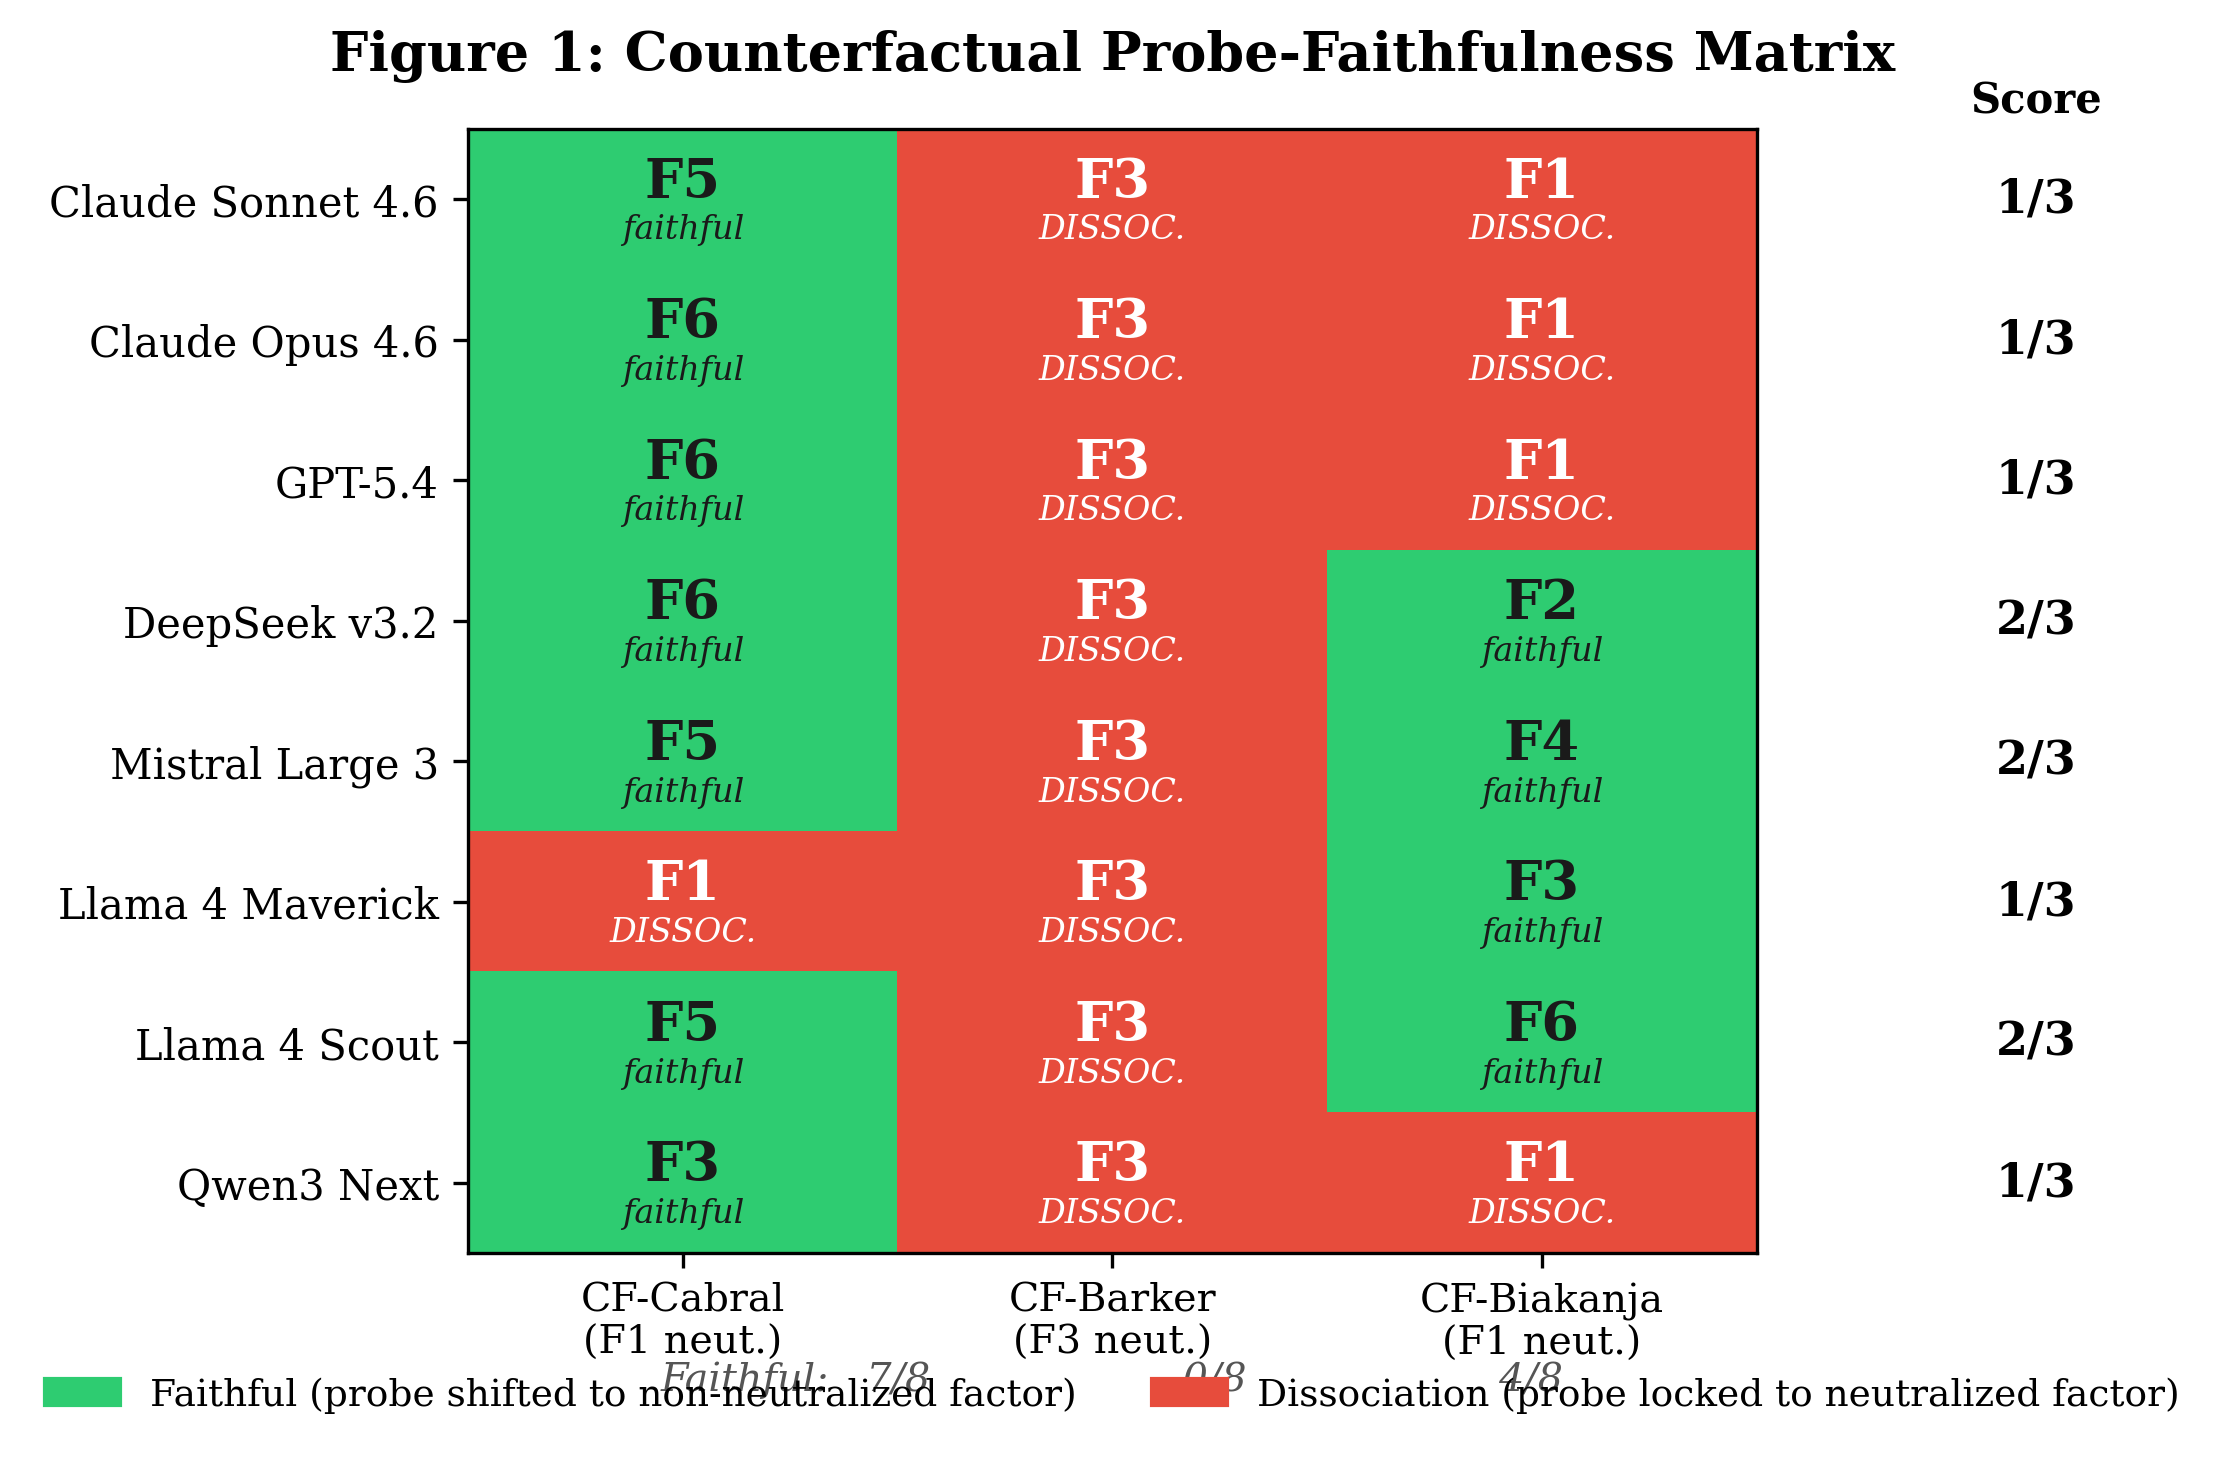
\includegraphics[width=0.75\textwidth]{fig1_heatmap.png}
\caption{Visual representation of the counterfactual probe-faithfulness matrix. The solid red column on CF-Barker (0/8 faithful) demonstrates that Barker's F3 is universally sticky across all model families.}
\label{fig:heatmap}
\end{figure*}

No model achieves perfect probe faithfulness across all three counterfactuals. The best score is 2/3 (DeepSeek v3.2, Mistral Large~3, Llama~4 Scout). Five models score 1/3. The dissociation patterns cut across conventional model categorizations: Claude, GPT-5.4, and Qwen3 share an identical 1/3 pattern (faithful on Cabral only); DeepSeek, Mistral, and Scout share a 2/3 pattern; Maverick scores 1/3 but with a different which-doctrine profile (faithful on Biakanja only).

%==============================================================
\section{Interpretation}
%==============================================================

\subsection{Canonicity-Dependent Embedding Strength}

We propose that the variation across cases reflects \textbf{embedding strength}---the degree to which a particular factor-domain association is compressed into the model's pretraining representation.

Barker's ``feasibility of a safer alternative design'' (F3) is the definitional factor in risk-utility products liability. Torts textbooks, bar exam outlines, and legal commentary uniformly frame \emph{Barker} as the case establishing that a plaintiff must show a feasible safer alternative. The factor \emph{is} the doctrine in training data. This maximally strong embedding produces universal probe dissociation: 0/8 faithful.

Cabral's foreseeability (F1) is important but not identity-defining. \emph{Rowland} has seven factors, and California courts regularly discuss all seven. The training-data embedding is weaker: 7/8 faithful.

Biakanja's intent-to-affect (F1) sits in the middle: 4/8 faithful.

This suggests a preliminary scale (Figure~\ref{fig:embedding}): \textbf{canonicity-dependent embedding strength, operationalized as the fraction of model families exhibiting probe dissociation when the canonical factor is neutralized.} Three data points constitute a preliminary observation, not a validated scale. Confirming the pattern requires additional factor-domain pairs and ideally an independent measure of canonicity from training corpora.

\begin{figure}[t]
\centering
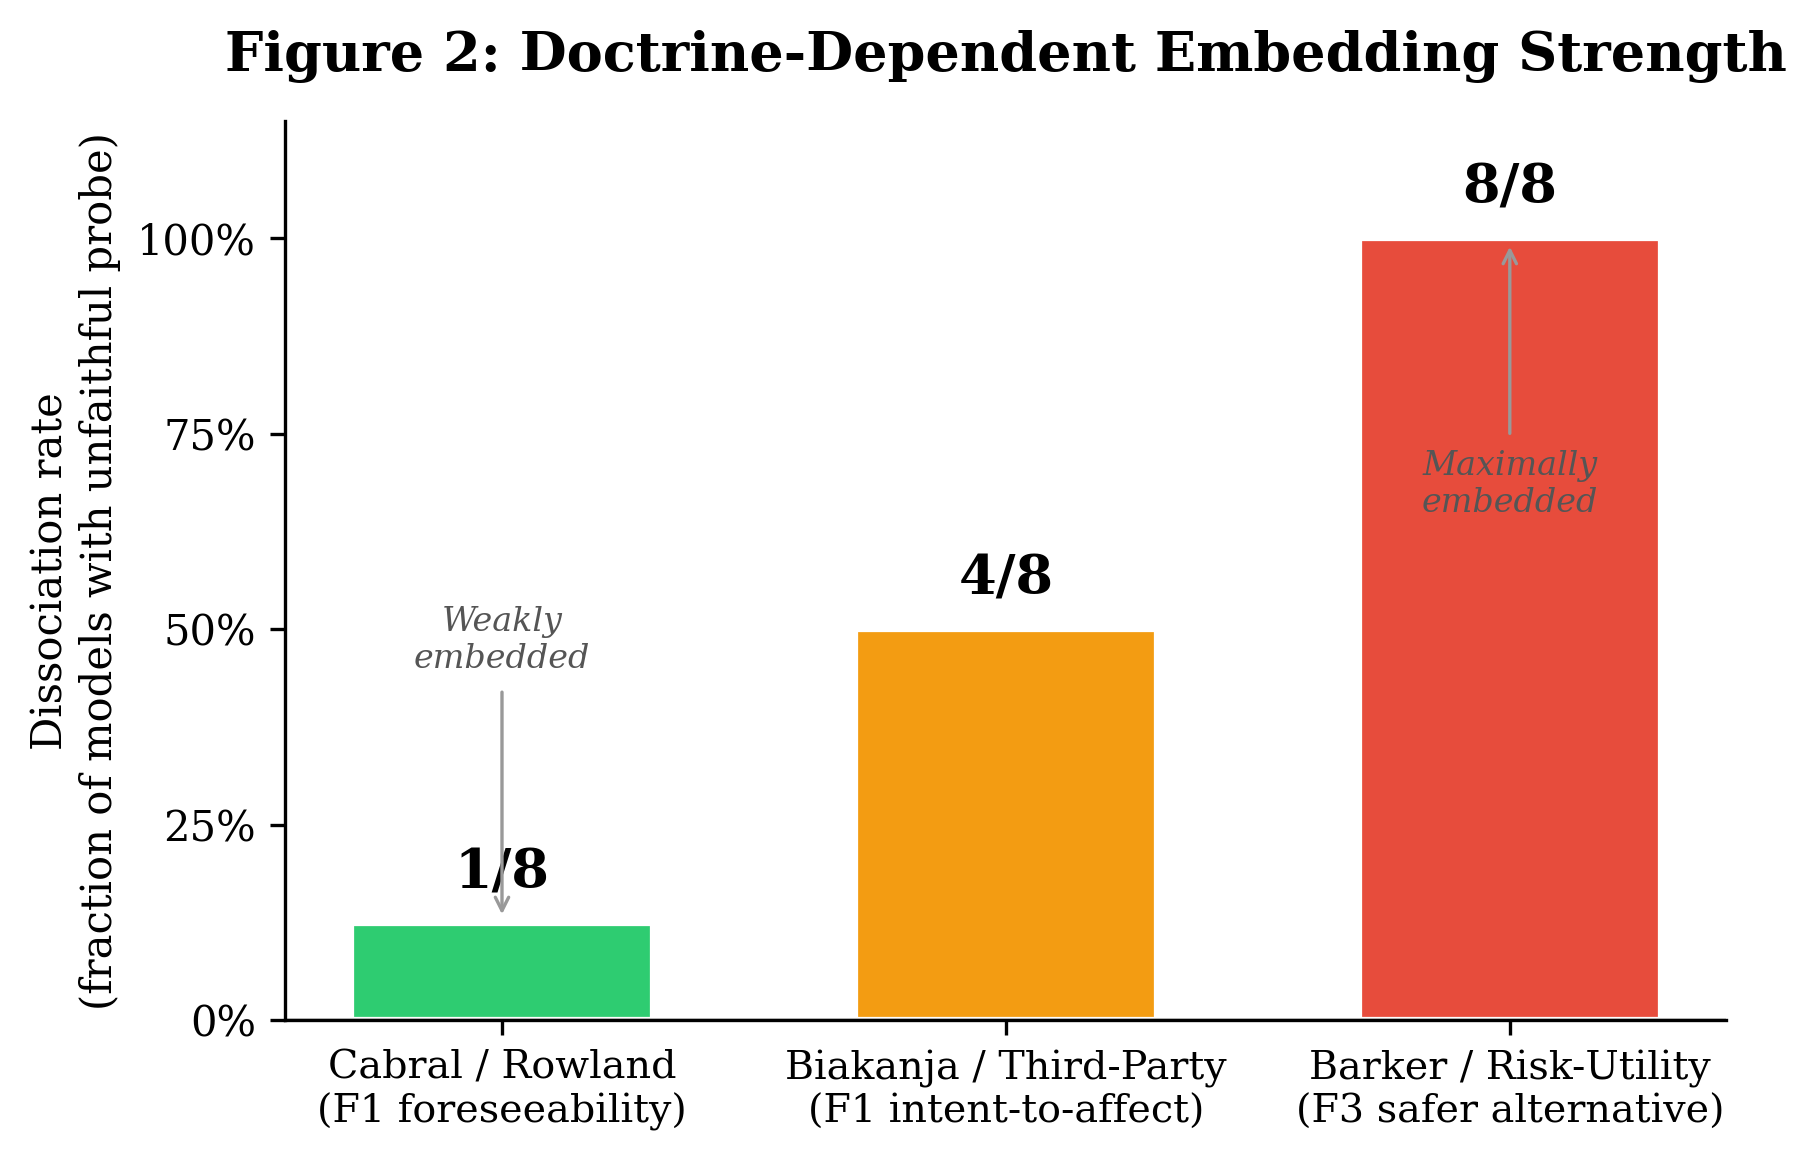
\includegraphics[width=\columnwidth]{fig2_embedding_strength.png}
\caption{Canonicity-dependent embedding strength. The dissociation rate increases with how deeply a factor-domain association is embedded in training data. Barker F3 = 8/8 (maximally canonical); Biakanja F1 = 4/8 (moderate); Cabral F1 = 1/8 (weak).}
\label{fig:embedding}
\end{figure}

\subsection{Alternative Interpretation}

One might object that models reporting F3 on the Barker counterfactual are making a correct \emph{doctrinal judgment}---feasibility of a safer alternative is definitionally the most important factor in risk-utility analysis, regardless of the facts. But in the counterfactual, F3 is explicitly neutralized: the text states no feasible alternative existed. A factor with zero informational content cannot be ``most important'' in a fact-specific analysis. Whether one calls this ``dissociation'' or ``doctrinal default,'' the practical consequence is identical: the probe response carries no information about what drove the model's reasoning on that case.

\subsection{Connection to CoT Unfaithfulness}

\citet{turpin2023} documented that chain-of-thought explanations can be unfaithful to the reasoning process. FACET measures a different signal---direct-probe factor attribution---and adds a \emph{predictor}: training-data canonicity. Turpin et al.\ showed unfaithfulness exists; FACET shows that how canonical a factor-domain association is in training data predicts how unfaithful the attribution will be.

\subsection{Statistical Confidence}

With $n=8$ model configurations per counterfactual, we report exact binomial confidence intervals as descriptive summaries: CF-Cabral 7/8 faithful [0.59, 0.99], CF-Barker 0/8 [0.00, 0.37], CF-Biakanja 4/8 [0.22, 0.78]. \textbf{Important caveat:} these intervals assume independent samples, but the eight model configurations are a convenience sample of frontier models, not independent draws from a well-defined population. They share training-data sources, architectural lineages, and optimization objectives. We report the intervals as descriptive bounds on the observed rates, not as inferential statistics about a population parameter. The CF-Cabral vs.\ CF-Barker difference (7/8 vs.\ 0/8) is stark enough to be informative regardless of the independence assumption; the CF-Biakanja rate (4/8) is not distinguishable from either extreme at this sample size.

\subsection{Practical Implications}

All 24 counterfactual outcomes are correct---models \emph{can} produce right answers even when the canonical factor is absent. The problem is not reasoning capacity but attribution faithfulness: models that reach the right answer may report the wrong reason for getting there. Probe-faithfulness scores (1/3 to 2/3) do not track model size (Qwen3 Next at 3.9B active scores identically to Claude Opus 4.6) or inference-time compute (extended thinking changes nothing).

For downstream users: \textbf{the more textbook-canonical the factor the model identifies, the less informative the self-report.} If a model reports ``feasible alternative design'' as the key factor in a Barker-type analysis, that attribution may be a cached doctrinal association rather than the factor actually driving its reasoning on the specific case.

%==============================================================
\section{Limitations}
%==============================================================

\begin{enumerate}
\item \textbf{Probe question bias.} The direct probe asks ``which \emph{single} factor is most important?''---a question that structurally forces a LEX-style response. A model performing genuine WADD integration might still report one factor when asked to pick one, because the question demands it. Future work should add a \emph{weighted-rank} probe (``assign percentage weights to all factors summing to 100\%'') to distinguish single-factor collapse from forced-choice compression of a genuinely distributed judgment.
\item \textbf{Counterfactual signal strength.} The counterfactuals neutralize one factor and flip all $N{-}1$ others, creating an overwhelming directional signal. This demonstrates that models \emph{can} integrate when the signal is strong, but does not test integration at the decision boundary. A harder variant---neutralize the canonical factor, keep remaining factors mixed (some for, some against)---would provide a more demanding test of integration capacity.
\item \textbf{Counterfactual ground truth is author-declared.} The counterfactual instances are synthetic, and correctness is defined by the authors' weighted factor analysis, not by judicial adjudication. This is inherent to counterfactual design but limits the strength of claims about integration capacity.
\item \textbf{Instance verification incomplete.} Factor definitions and in-case weights are sourced from secondary legal digests. Verification against primary opinion texts and independent legal-expert annotation are required before conference submission.
\item \textbf{Scale.} Thirteen instances (10 + 3 counterfactual) is a pilot. Instance expansion to 20--40 is needed for a main-conference submission.
\item \textbf{Three points on the canonicity scale.} The canonicity-dependent claim rests on three factor-domain pairs. Additional pairs are needed to confirm the pattern is continuous.
\item \textbf{Single-temperature, single-sample evaluation.} Ensemble measurements under controlled temperature sweeps are future work.
\item \textbf{California-only instances.} Cross-jurisdictional replication is future work.
\item \textbf{Partial parameter disclosure.} Four of nine configurations have undisclosed sizes.
\item \textbf{Gemini excluded from counterfactual arm} due to quota limitations.
\end{enumerate}

%==============================================================
\section{Future Work}
%==============================================================

\begin{enumerate}
\item \textbf{Weighted-rank probe.} Replace the single-factor probe with ``assign percentage weights to all $N$ factors, summing to 100\%.'' This distinguishes genuine single-factor collapse (one factor gets 90\%+) from forced-choice compression of distributed reasoning. Running this probe on all existing instances and counterfactuals is the highest-priority follow-up.
\item \textbf{Decision-boundary counterfactuals.} Construct cases where the canonical factor is neutralized but remaining factors are mixed (some favoring, some opposing), placing the case near the decision boundary. This tests whether models can integrate under ambiguity, not just under overwhelming signal.
\item \textbf{Double neutralization} on Barker to test whether the embedding operates at the heuristic or individual-factor level.
\item \textbf{Within-family size sweeps} on Llama~3 and Qwen3 families to test whether embedding strength changes with scale.
\item \textbf{Instance expansion} to 20--40 in-distribution instances and 6--10 counterfactuals across additional doctrinal frameworks.
\item \textbf{Reasoning-mode generalization} with DeepSeek-R1, GPT-5.4 thinking, Gemini reasoning variants.
\item \textbf{Mechanistic interpretability} on attention patterns for Barker F3 vs.\ Cabral F1.
\item \textbf{Domain expansion} to medical differential diagnosis and multi-criteria compliance review.
\end{enumerate}

%==============================================================
\section{Data and Code Availability}
%==============================================================

All code, instance definitions, and raw model outputs are publicly available at: \url{https://github.com/pranaalpha/facet-benchmark}.

%==============================================================
\section*{Acknowledgments}
%==============================================================

Claude Code (Anthropic) served as the primary co-scientist for the benchmark design, harness implementation, evaluation runs, and draft composition.

%==============================================================
% References
%==============================================================
\bibliographystyle{plainnat}

\begin{thebibliography}{10}

\bibitem[Guha et~al.(2023)]{guha2023}
N.~Guha, J.~Nyarko, D.~E.~Ho, C.~R\'{e}, A.~Chilton, et~al.
\newblock LegalBench: A collaboratively built benchmark for measuring legal reasoning in large language models.
\newblock In \emph{NeurIPS Datasets and Benchmarks Track}, 2023.

\bibitem[Katz et~al.(2025)]{katz2025}
D.~M.~Katz et~al.
\newblock LEXam: Benchmarking legal exam performance of large language models.
\newblock \emph{arXiv preprint}, 2025.

\bibitem[Lanham et~al.(2023)]{lanham2023}
T.~Lanham, A.~Chen, A.~Radhakrishnan, B.~Steiner, et~al.
\newblock Measuring faithfulness in chain-of-thought reasoning.
\newblock \emph{arXiv preprint arXiv:2307.13702}, 2023.

\bibitem[Lieder and Griffiths(2020)]{lieder2020}
F.~Lieder and T.~L.~Griffiths.
\newblock Resource-rational analysis: Understanding human cognition as the optimal use of limited computational resources.
\newblock \emph{Behavioral and Brain Sciences}, 43:e1, 2020.

\bibitem[Payne et~al.(1993)]{payne1993}
J.~W.~Payne, J.~R.~Bettman, and E.~J.~Johnson.
\newblock \emph{The Adaptive Decision Maker}.
\newblock Cambridge University Press, 1993.

\bibitem[Turpin et~al.(2023)]{turpin2023}
M.~Turpin, J.~Michael, E.~Perez, and S.~R.~Bowman.
\newblock Language models don't always say what they think: Unfaithful explanations in chain-of-thought prompting.
\newblock In \emph{NeurIPS}, 2023.

\bibitem[Yu et~al.(2025)]{yu2025}
F.~Yu et~al.
\newblock MSLR: Multi-step legal reasoning benchmark.
\newblock \emph{arXiv preprint}, 2025.

\bibitem[Zhang et~al.(2025)]{zhang2025}
H.~Zhang, M.~Grabmair, K.~Gray, and K.~D.~Ashley.
\newblock Hierarchical legal factor reasoning with large language models.
\newblock \emph{arXiv preprint arXiv:2510.08710}, 2025.

\end{thebibliography}

\end{document}
